\chapter{Il Dataset TON\_IoT}

Il dataset \textit{Ton\_IoT} rappresenta uno dei principali dataset utilizzati per l'addestramento e la valutazione dei modelli di \textit{Intrusion Detection System (IDS)}. È stato sviluppato dall'Università del New South Wales (UNSW) a Canberra ed è stato progettato per simulare scenari realistici di rete IoT. Il dataset è stato generato tramite un testbed complesso, che include vari livelli di interazione tra i dispositivi \textit{edge}, \textit{fog} e \textit{cloud}, emulando le comunicazioni tipiche dei sistemi IoT moderni.

Una delle ragioni della sua ampia diffusione è la sua natura estremamente eterogenea: \textit{Ton\_IoT} contiene dati di telemetria provenienti dai dispositivi IoT, dati estratti dai sistemi operativi (sia Windows che Linux) e dati relativi al traffico di rete. Questa caratteristica lo distingue da molti altri dataset nel campo della sicurezza informatica. Il nome stesso \textit{Ton\_IoT} deriva proprio dall'acronimo di \textit{Telemetry, Operating Systems, and Network Internet of Things}, riflettendo la varietà e la completezza delle fonti di dati incluse. \cite{Ton_IoT}

\section{Architettura del dataset}

L'architettura del dataset \textit{Ton\_IoT} è stata sviluppata per rappresentare una rete IoT complessa, distribuita su tre livelli principali: \textbf{edge}, \textbf{fog} e \textbf{cloud}. Questa struttura è stata implementata utilizzando tecnologie avanzate come \textit{Software-Defined Networking (SDN)}, \textit{Network Function Virtualization (NFV)} e \textit{Service Orchestration (SO)}.

\begin{itemize}
    \item \textbf{Livello Edge}: Questo livello è composto da dispositivi fisici IoT/IIoT che eseguono operazioni di rete, raccolgono dati sensoriali e comunicano con lo strato fog e cloud. Dispositivi come sensori per il monitoraggio ambientale, smart TVs e smartphones sono gestiti da gateway locali che indirizzano i dati verso lo strato fog.
    
    \item \textbf{Livello Fog}: Il livello fog integra la virtualizzazione delle funzioni di rete, utilizzando macchine virtuali (VMs) per l'analisi dei dati vicino alla sorgente. In questo contesto, le macchine virtuali distribuiscono i carichi di lavoro, eseguendo analisi preliminari e riducendo la latenza e la dipendenza dal cloud. La piattaforma VMware NSX è stata utilizzata per gestire le comunicazioni e la segmentazione della rete tra i vari livelli.
    
    \item \textbf{Livello Cloud}: Il livello cloud include servizi online, come il monitoraggio remoto dei dati e l'analisi approfondita del traffico di rete e dei dati IoT. Questo strato è responsabile dell'elaborazione di grandi volumi di dati provenienti dagli strati edge e fog. Servizi cloud come Microsoft Azure o AWS sono stati utilizzati per immagazzinare e processare i dati raccolti.
\end{itemize}

\begin{figure}[htbp]
\centering
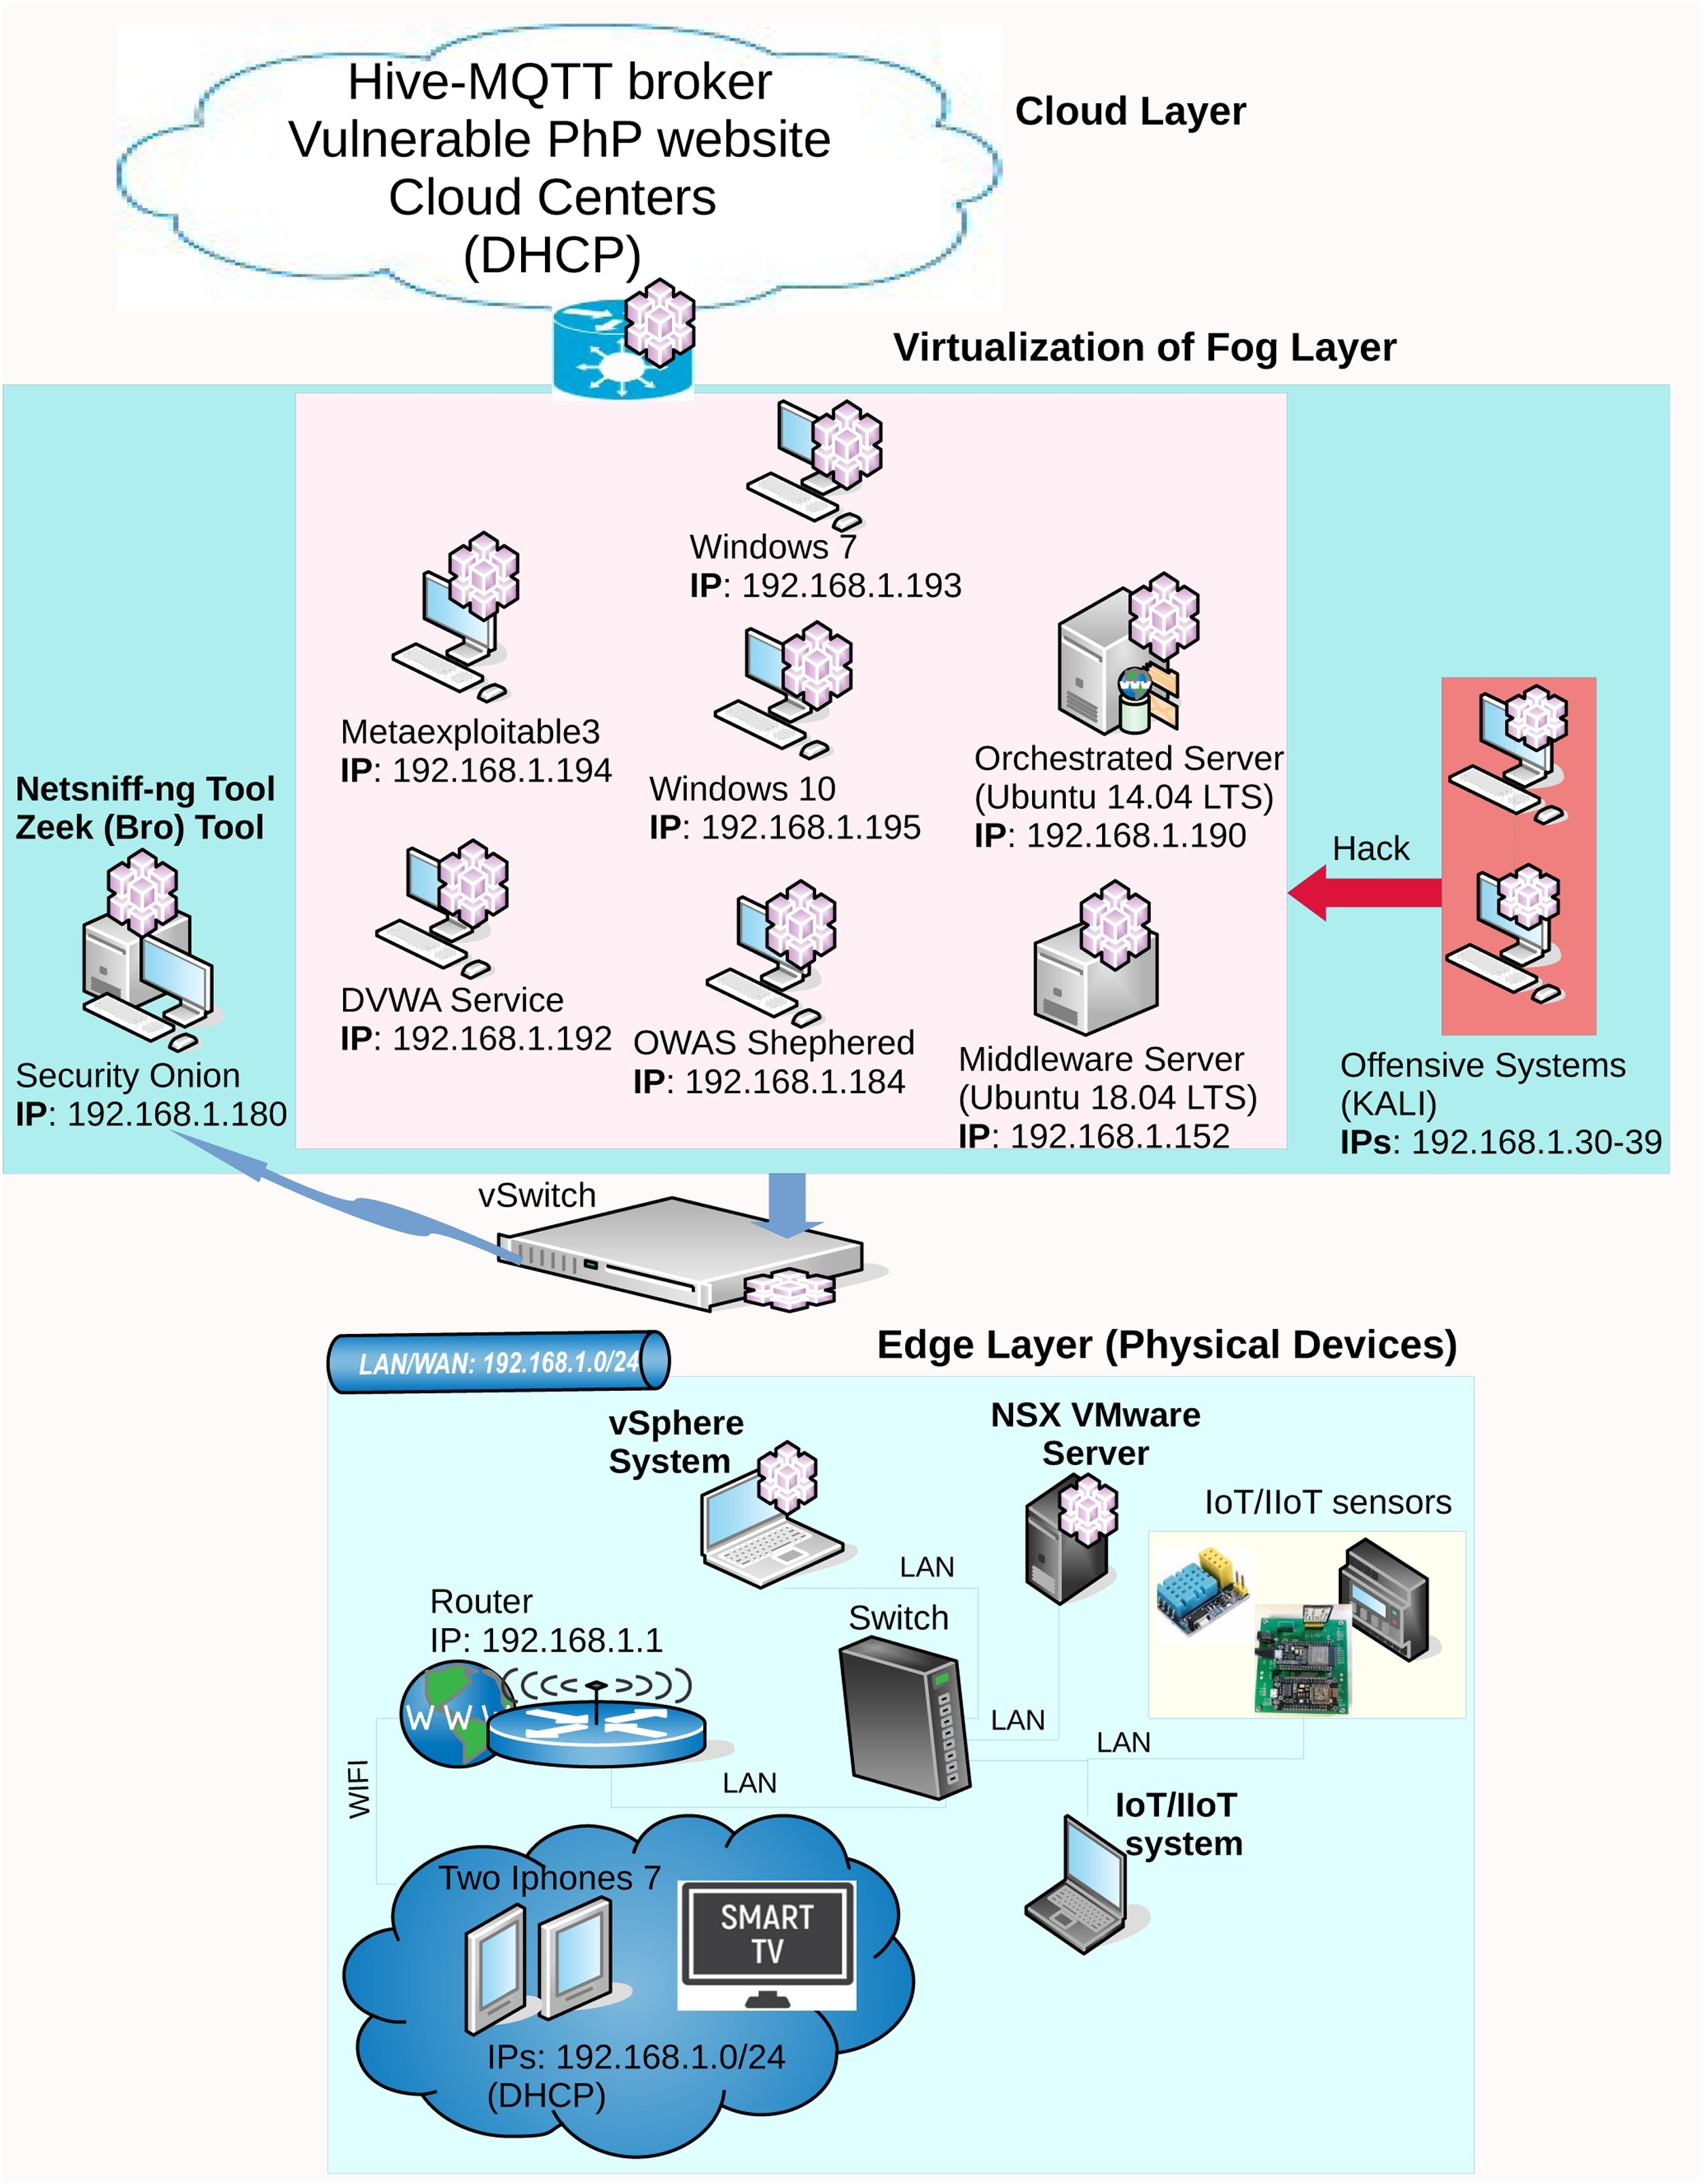
\includegraphics[scale= 0.7]{UNINA_MSc_Thesis_Project/img/Ton_Architecture.jpg}
  \caption{Architettura Ton IoT Dataset}
\end{figure}



\section{Tecnologie di supporto}

Le tecnologie alla base di questo testbed sono fondamentali per la flessibilità e la dinamicità delle interazioni tra i vari livelli:

\begin{itemize}
    \item \textbf{SDN (Software-Defined Networking)}: Consente di configurare in modo dinamico la rete tramite la programmabilità. Questa tecnologia è implementata tramite la piattaforma NSX-VMware, che permette di creare reti virtuali sovrapposte con funzionalità equivalenti a quelle fisiche.
    
    \item \textbf{NFV (Network Function Virtualization)}: Riduce la necessità di hardware specializzato sostituendo dispositivi fisici con funzioni di rete basate su software, eseguite come macchine virtuali. In questo modo, è possibile implementare scenari di attacco e normali all'interno del testbed.
    
    \item \textbf{SO (Service Orchestration)}: Gestisce l'orchestrazione dei servizi di rete, consentendo la distribuzione automatica delle risorse tra i vari livelli. L'integrazione di SO migliora l'efficienza operativa e garantisce la gestione dinamica dei flussi di dati tra edge, fog e cloud.
\end{itemize}

Questa architettura consente di raccogliere dati da diverse fonti eterogenee e offre un ambiente flessibile e realistico per valutare la capacità degli \textit{Intrusion Detection Systems (IDS)} di rilevare attacchi in ambienti distribuiti.

\section{Scenari di Attacco e Normali}

Il dataset \textit{Ton\_IoT} include sia traffico benigno che scenari di attacco. Gli scenari normali sono stati generati attraverso operazioni legittime che coinvolgono servizi IoT/IIoT come FTP, DNS e HTTP, simulati nel testbed. Gli scenari di attacco includono nove famiglie di attacchi: \textit{Denial of Service (DoS)}, \textit{Distributed Denial of Service (DDoS)}, \textit{injection}, \textit{Man-in-the-Middle (MITM)}, \textit{password cracking}, \textit{ransomware}, \textit{scanning}, \textit{XSS} e \textit{backdoor}. Ogni attacco è stato lanciato contro vulnerabilità specifiche nei servizi IoT/IIoT o nei sistemi operativi ospitati.

\section{Motivazione per l'Uso del Ton\_IoT nella Tesi}

Il dataset \textit{Ton\_IoT} è stato scelto per questo lavoro di tesi per la sua capacità di rappresentare scenari realistici che coinvolgono interazioni tra dispositivi IoT/IIoT e sistemi di rete distribuiti. Una delle caratteristiche principali del dataset è la raccolta di dati eterogenei da quattro fonti: traffico di rete, telemetria dei dispositivi IoT, tracce di audit di sistemi operativi (Windows e Linux), e dati di attacco generati da scenari di hacking simulati. Questo lo rende particolarmente adatto per valutare l'efficacia di sistemi di \textit{Intrusion Detection System (IDS)} basati su tecniche di \textit{machine learning} in ambienti IoT, che rappresentano il focus centrale di questo lavoro di tesi.

Inoltre, la struttura del dataset permette di esplorare come differenti livelli di simulazione e attacchi distribuiti possano influenzare la capacità di generalizzazione degli \textit{IDS}.

\section{Caratteristiche Principali del Dataset}

Il dataset è suddiviso in vari file in formato CSV e pcap che contengono i dati etichettati relativi agli attacchi e ai normali scenari di rete. Ogni file contiene 44 attributi, che descrivono varie caratteristiche del traffico di rete e delle operazioni di sistema. Sono inoltre presenti etichette che indicano se il record rappresenta un comportamento normale o un attacco, e in caso di attacco, il tipo specifico di attacco. Questi dati sono stati utilizzati per addestrare e testare diversi modelli di apprendimento automatico durante gli esperimenti di questa tesi.

